%% LyX 2.3.1 created this file.  For more info, see http://www.lyx.org/.
%% Do not edit unless you really know what you are doing.
\documentclass[english,osajnl,jcp,reprint,groupedaddress,noshowpacs,showkeys,longbibliography,noeprint,nofootinbib,bibtex,ruled,vlined,english,natural,table,usenames,dvipsnames,a4paper]{revtex4-1}
\usepackage[T1]{fontenc}
\usepackage[utf8]{inputenc}
\setcounter{secnumdepth}{3}
\usepackage{color}
\usepackage{babel}
\usepackage{array}
\usepackage{booktabs}
\usepackage{mathtools}
\usepackage{amsmath}
\usepackage{amssymb}
\usepackage{graphicx}
\usepackage{microtype}
\usepackage[unicode=true,
bookmarks=false,
breaklinks=false,pdfborder={0 0 1},backref=section,colorlinks=true]
{hyperref}
%\hypersetup{%
%	linkcolor=BrickRed,urlcolor=blue!50!black,citecolor=blue!50!black}

\makeatletter

%%%%%%%%%%%%%%%%%%%%%%%%%%%%%% LyX specific LaTeX commands.
%% Because html converters don't know tabularnewline
\providecommand{\tabularnewline}{\\}

%%%%%%%%%%%%%%%%%%%%%%%%%%%%%% User specified LaTeX commands.
\usepackage{siunitx}

\newcommand*\samethanks[1][\value{footnote}]{\footnotemark[#1]}

%\author[1]{Moritz Hoffmann\thanks{Equal contributions}}
%\author[1]{Christoph Fröhner\samethanks}
%\author[1]{Frank Noé\thanks{Corresponding author}}
%\affil[1]{Freie Universität Berlin, Fachbereich Mathematik und Informatik,\newline Arnimallee 6, 14195 Berlin, Germany}
%\affil[ ]{\textit{\{ moritz.hoffmann,christoph.froehner,frank.noe \}@fu-berlin.de}}


\newlength{\singlecolumnwidth}
\newlength{\doublecolumnwidth}
\singlecolumnwidth=3.37in
\doublecolumnwidth=6.69in

\makeatother

\linespread{0.956}

\newif\ifthisispreprint
% \thisispreprinttrue
\thisispreprintfalse

\begin{document}
	
	\author{Moritz Hoffmann}
	\email{moritz.hoffmann@fu-berlin.de}
	\thanks{Equal contributions}
	\affiliation{
		Freie Universität Berlin, Fachbereich Mathematik und Informatik,
		Arnimallee 6, 14195 Berlin, Germany
	}
	
	\author{Christoph Fröhner}
	\email{christoph.froehner@fu-berlin.de}
	\thanks{Equal contributions}
	\affiliation{
		Freie Universität Berlin, Fachbereich Mathematik und Informatik,
		Arnimallee 6, 14195 Berlin, Germany
	}
	
	\author{Frank Noé}
	\email{frank.noe@fu-berlin.de}
	\thanks{Corresponding author}
	\affiliation{
		Freie Universität Berlin, Fachbereich Mathematik und Informatik,
		Arnimallee 6, 14195 Berlin, Germany
	}
	
	
\title{Reactive SINDy: Discovering governing reactions from concentration
data}

\begin{abstract}
The inner workings of a biological cell or a chemical reaction can
be rationalized by the network of reactions, whose structure reveals
the most important functional mechanisms. For complex systems, these
reaction networks are not known a priori and cannot be efficiently
computed with \emph{ab initio} methods, therefore an important approach
goal is to estimate effective reaction networks from observations,
such as time series of the main species. Reaction networks estimated
with standard machine learning techniques such as least-squares regression
may fit the observations, but will typically contain spurious reactions.
Here we extend the sparse identification of nonlinear dynamics (SINDy)
method to vector-valued ansatz functions, each describing a particular
reaction process. The resulting sparse tensor regression method ``reactive
SINDy'' is able to estimate a parsimonious reaction network. We illustrate
that a gene regulation network can be correctly estimated from observed
time series.
\end{abstract}

\maketitle

\section{Introduction}

Mapping out the reaction networks behind biological processes, such
as gene regulation in cancer~\cite{Abramovitch2004}, is paramount
to understanding the mechanisms of life and disease. A well-known
example of gene regulation is the lactose operon whose crystal structure
was resolved in~\cite{Lewis1996} and dynamics were modeled in~\cite{Yildirim2003}.
The system's ``combinatorial control'' in E. coli cells was quantitatively
investigated in~\cite{Kuhlman2007}, in particular studying repression
and activation effects. These gene regulatory effects often appear
in complex networks~\cite{Shen-Orr2002} and there exist databases
resolving these for certain types of cells, e.g., E. coli cells~\cite{Gama-Castro2016}
and yeast cells~\cite{Lee2002}. Another example where mapping the
active reactions is important is that of chemical reactors~\cite{Roa2017},
where understanding which reactions are accessible for a given set
of educts and reaction conditions is important to design synthesis
pathways~\cite{cong1999high,kiwi2005microstructured}.

The traditional approach to determine a reaction network is to propose
the structure of the network based on chemical insight and subsequently
fit the parameters given available data~\cite{schoneberg2014explicit}.
To decipher complex reaction environments such as biological cells,
it would be desirable to have a data-driven approach that can answer
the question which reactions are underlying a given observation, e.g.,
the time series of a set of reactants. However, in sufficiently complex
reaction environments the number of reactive species and possible
reactions is practically unlimited -- as an illustration, consider
vast amount of possible isomerizations and post-translational modifications
for a single protein molecule. Therefore, the more specific formulation
is ``given observations of a set of chemical species, what is the
\emph{minimal set} of reactions necessary to explain their time evolution?''.
This formulation calls for a machine learning method that can infer
the reaction network underlying the observation data.

Knowledge about the reaction network can be applied to parameterize
other numerical methods to further investigate the processes at hand.
Such methods include particle-based approaches derived from the chemical
master equation~\cite{gillespie1977exact,winkelmann2016spatiotemporal,winkelmann2017hybrid,isaacson2009reaction},
as well as highly detailed but parameter-rich methods such as particle-based
or interacting-particle reaction~dynamics~\cite{schoneberg2013readdy,hoffmann2018readdy,frohner2018reversible,donev2018efficient,Andrews2017,van2005green,van2005simulating}
capable of fully resolving molecule positions in space and time --
see~\cite{schoneberg2014simulation,Andrews2018} for recent reviews.

Existing methods to infer regulatory networks include ARCANE~\cite{Margolin2006}
that uses experimental essay data and information theory, as well
as the likelihood approach presented in~\cite{Tian2007a} that takes
the stochasticity of observed reactant time series into account.

The method presented in this work can identify underlying complex
reaction networks from concentration time series by following the
law of parsimony, i.e., by inducing sparsity in the resulting reaction
network. This promotes the interpretability of the model and avoids
overfitting. We formulate the problem as data-driven identification
of a dynamical system, which renders the method consistent with and
an extension of the framework of sparse identification of nonlinear
dynamics (SINDy)~\cite{Brunton2015}. Specifically, the problem of
identifying a reaction network from time traces of reactant concentrations
can be solved by finding a linear combination from a library of candidate
nonlinear functions (ansatz functions) that each corresponds to a reaction acting on a set
of reactants. With this formulation, the reaction rates can be determined
\emph{via} regression. Sparsity is induced by equipping the regression
algorithms with a sparsity inducing regularization. SINDy was investigated,
generalized, and applied in many different ways, e.g., including control~\cite{brunton2016sparse}
(SINDYc), in the context of partial differential equations~\cite{rudy2017data},
updating already existing models~\cite{quade2018sparse} (abrupt-SINDy),
and looking into convergence properties~\cite{zhang2018convergence}.

We extend and apply SINDy to the case of learning reaction networks
from non-equilibrium concentration data. Similar approaches make use
of SINDy but do not resolve specific reactions~\cite{mangan2016inferring},
use weak formulations to avoid numerical temporal derivatives~\cite{pantazis2017unified},
or use compressive sensing and sparse Bayesian learning~\cite{Pan2012}.

Our extension of the original SINDy method mostly involves estimating
parameters which are coupled across the equations of the arising dynamical
system. In the context of learning reaction networks this means that
we look for specific reactions and their rate constants that might
have lead to the observations instead of net flux across species.
We demonstrate the algorithm on a gene regulatory network in three
different scenarios of measurement: When there is no noise in the
data we can find, given sufficient amounts of data, all relevant processes
of the ground truth. If there is noise in the data we converge to
the correct reaction network and rates with decreasing levels of noise.
The third scenario generalizes the method to two measurements with
different initial conditions, also converging to the correct model
with decreasing levels of noise.

We additionally demonstrate the algorithm
on time series data of the mitogen activated protein kinases (MAPK) pathway as 
an example for a bimodal system and on time series data of the
Lotka-Volterra system which describes oscillatory predator-prey dynamics subject to
social friction. In both systems reactive SINDy recovers the generating 
reaction network whereas non-sparse estimation detects many false processes.

\section{Reactive SINDy: Sparse learning of reaction kinetics}

We are observing the concentrations of $S$ chemical species in time
$t$: 
\begin{align}
\mathbf{x}(t)=\begin{pmatrix}x_{1}(t)\\
\vdots\\
x_{S}(t)
\end{pmatrix}\in\mathbb{R}^{S}.\label{eq:concentration_vector}
\end{align}
We assume that their dynamics are governed by classical reaction-rate
equations subject to the law of mass action. A general expression
for the change of concentration of reactant $s$ as a result of order-0
reactions (creation or annihilation), order-1 reactions (transitions
of other species into $s$ or transitions of $s$ into other species),
order-2 reactions (production or consumption of $s$ by the encounter
of two species), etc, is given by:

\begin{equation}
\dot{x}_{s}=\sum_{i}\beta_{s,0}^{(i)}+\sum_{i}\beta_{s,1}^{(i)}x_{i}+\sum_{i,j}\beta_{s,2}^{(i,j)}x_{i}x_{j}+\ldots\label{eq:lma}
\end{equation}
where the $\beta_{s,k}^{(\ldots)}$-values are constants belonging
to the reactions of order $k$. These rate constants however can incorporate
several underlying reactions at once. For example, the two reactions
\begin{align}
s_{1}\xrightharpoonup{\xi_{1}}s_{2}\label{eq:example_reaction_1}\\
s_{1}\xrightharpoonup{\xi_{2}}s_{3}\label{eq:example_reaction_2}
\end{align}
both contribute to $\dot{x}_{1}=\beta_{1,1}^{(1)}x_{1}=-(\xi_{1}+\xi_{2})x_{1}$.
To disentangle (\ref{eq:lma}) into single reactions, we choose a
library of $R$ possible ansatz reactions that each represent a single
reaction: 
\begin{align}
\textbf{y}_{r}(\textbf{x}(t))=\begin{pmatrix}y_{r,1}(\textbf{x}(t))\\
\vdots\\
y_{r,S}(\textbf{x}(t))
\end{pmatrix},\quad r=1,\ldots,R.
\end{align}
With this ansatz, the reaction dynamics (\ref{eq:lma}) becomes a
set of linear equations with unknown parameters $\xi_{r}$ that represent
the sought macroscopic rate constants: 
\begin{align}
\dot{\textbf{x}}_{i}(t)=\sum_{r=1}^{R}y_{r,i}(\textbf{x}(t))\xi_{r},\quad i=1,\ldots,S,\label{method:the-system}
\end{align}
where $\xi_{r}$ are the to-be estimated macroscopic rate constants.
The two reactions in the previous example (\ref{eq:example_reaction_1}-\ref{eq:example_reaction_2})
would be modeled by the functions
\begin{align*}
y_{1}(\mathbf{x}) & =(-x_{1},x_{1},0)^{\top},\\
y_{2}(\mathbf{x}) & =(-x_{1},0,x_{1})^{\top},
\end{align*}
illustrating that the values of the coefficients $\xi_{1}$ and $\xi_{2}$
can be used to decide whether a single reaction is present and to
what degree.

Now suppose we have measured the concentration vector (\ref{eq:concentration_vector})
at $T$ time points $t_{1}<\cdots<t_{T}$. We represent these data
as a matrix 
\begin{align}
\textbf{X}=\left(\begin{array}{cccc}
\mathbf{x}(t_{1}) & \mathbf{x}(t_{2}) & \cdots & \mathbf{x}(t_{T})\end{array}\right)^{\top}\in\mathbb{R}^{T\times S}.
\end{align}
Given this matrix, a library $\Theta:\mathbb{R}^{T\times S}\to\mathbb{R}^{T\times S\times R},\;\mathbf{X}\mapsto\begin{pmatrix}\theta_{1}(\mathbf{X}) & \theta_{2}(\mathbf{X}) & \cdots & \theta_{R}(\mathbf{X})\end{pmatrix}$
of $R$ candidate (ansatz) reactions can be proposed with corresponding reaction
functions 
\begin{align}
\theta_{r}(\mathbf{X})=\begin{pmatrix}\textbf{y}_{r}(\mathbf{X}_{1*})^{\top}\\
\vdots\\
\textbf{y}_{r}(\mathbf{X}_{T*})^{\top}
\end{pmatrix}\in\mathbb{R}^{T\times S},\quad r=1,\ldots,R,\label{method:the-reactions}
\end{align}
where $\textbf{X}_{i*}$ denotes the $i$-th row in $\textbf{X}$.
Applying the concentration trajectory to the library yields $\Theta(\textbf{X})\in\mathbb{R}^{T\times S\times R}$. 

The goal is to find coefficients $\Xi=\begin{pmatrix}\xi_{1} & \xi_{2} & \cdots & \xi_{R}\end{pmatrix}^{\top}$,
so that 
\begin{align}
\dot{\textbf{X}}=\Theta(\textbf{X})\Xi=\sum_{r=1}^{R}\theta_{r}(\textbf{X})\xi_{r}.
\end{align}
In particular, the system is linear in the coefficients $\Xi$, which
makes regression tools such as elastic net regularization~\cite{Zou2005}
applicable. To this end, one can consider the regularized minimization
problem (reactive SINDy): 
\begin{align}
\hat{\Xi}&=\underset{\Xi}{\arg\min}\Bigg(\frac{1}{2T}\left\Vert \dot{\textbf{X}}-\Theta(\textbf{X})\Xi\right\Vert _{F}^{2} \label{method:minimizationproblem} \\
&\quad+\alpha\lambda\|\Xi\|_{1}+\alpha(1-\lambda)\|\Xi\|_{2}^{2}\Bigg)\quad\text{subject to }\Xi\geq0.\nonumber
\end{align}
Here, $\|\cdot\|_{F}$ denotes the Frobenius norm, $\lambda\in[0,1]$
is a hyperparameter that interpolates linearly between LASSO~\cite{Tibshirani1996,Hastie2009}
and Ridge~\cite{Hoerl1} methods, and $\alpha\geq0$ is a hyperparameter
that, depending on $\lambda$, can induce sparsity and give preference
to smaller solutions in the $L_{1}$ or $L_{2}$ sense. For $\alpha=0$
the minimization problem reduces to standard least-squares (LSQ) with
the constraint $\Xi\geq0$. Reactive SINDy (\ref{method:minimizationproblem})
is therefore a generalization of the SINDy method to vector-valued
ansatz functions.

Since only the concentration data $\mathbf{X}$ is available but not
its temporal derivative, $\dot{\mathbf{X}}$ is approximated numerically
by second order finite differences with the exception of boundary
data. Once the pair $(\mathbf{X},\dot{\mathbf{X}})$ is obtained,
the problem becomes invariant under temporal reordering. Hence, when
presented with multiple trajectories the data matrices $\mathbf{X}_{i}$
and $\dot{\mathbf{X}}_{i}$ can simply be concatenated.

In order to solve (\ref{method:minimizationproblem}) the numerical
sequential least-squares minimizer SLSQP~\cite{Kraft1988} is applied
via the software package SciPy~\cite{SciPy}. Code related to this
paper can be found under \url{https://github.com/readdy/readdy_learn}. 

\section{Results\label{sec:results}}

We demonstrate the method by estimating the reactions of a gene-regulatory
network from time series of concentrations of the involved molecules.
Let $S:=\{A,B,C\}$ be a set of three species of proteins which are
being translated each from their respective $\mathrm{mRNA}$ molecule.
Each $\mathrm{mRNA}$ in turn has a corresponding $\mathrm{DNA}$
which it is transcribed from. The proteins and $\mathrm{mRNA}$ molecules
decay over time whereas the $\mathrm{DNA}$ concentration remains
constant. The network contains reactions of the following form~\cite{Thattai2001a}
\begin{align*}
\mathrm{DNA}_{i} & \rightharpoonup\mathrm{DNA}_{i}+\mathrm{mRNA}_{i} &  & \text{(transcription)},\\
\mathrm{mRNA}_{i} & \rightharpoonup\mathrm{mRNA}_{i}+i &  & \text{(translation)},\\
\mathrm{mRNA}_{i} & \rightharpoonup\emptyset &  & \text{(decay of mRNA)},\\
i & \rightharpoonup\emptyset &  & \text{(decay of protein)},\\
i+\mathrm{mRNA}_{j} & \rightharpoonup i &  & \text{(regulation of }j\in S\text{),}
\end{align*}
for each of the species $i\in S$. These reactions model a regulation
of species $j$ by virtue of the fact that the transcription product
inhibits the transcription processes. In our example proteins of type
$\mathrm{A}$ regulate the $\mathrm{mRNA}_{\mathrm{B}}$ molecules,
proteins of type $\mathrm{B}$ regulate the $\mathrm{mRNA}_{\mathrm{C}}$
molecules and proteins of type $\mathrm{C}$ regulate the $\mathrm{mRNA}_{\mathrm{A}}$
molecules (Fig.~\ref{fig:network}). Using this reaction model, time
series of concentrations are generated using the rates given in Tab~\ref{tab:reaction-library}
under the initial condition described in Tab~\ref{tab:Initial-conditions}a,
which were chosen so that all the reactions in the reaction model
significantly contribute to the temporal evolution of the system's
concentrations. The generation samples the integrated equations equidistantly
with a discrete time step of $\tau=3\cdot10^{-3}$ yielding $667$
frames which amounts to a cumulative time of roughly $T=2$.

\begin{figure}[h!]
\centering 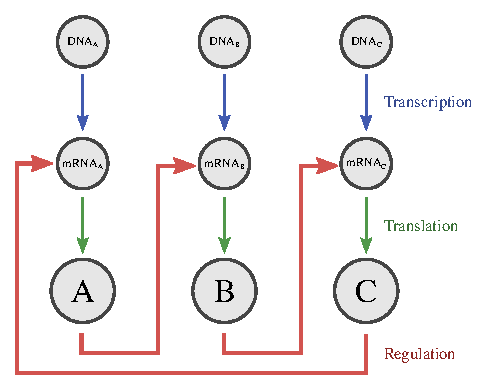
\includegraphics[width=\singlecolumnwidth]{figures_jcp/1.pdf}
\caption{\label{fig:network}The regulation network example described in Sec.~\ref{sec:results}.
Each circle depicts a species, each arrow corresponds to one reaction.
Blue arrows denote transcription from $\mathrm{DNA}$ to $\mathrm{mRNA}$,
green arrows denote translation from $\mathrm{mRNA}$ to protein,
and red arrows denote the regulatory network.}
\end{figure}
\begin{table}
\centering%
\ifthisispreprint
% ignore
\else
\resizebox{.95\columnwidth}{!}{%
\fi
\begin{tabular}{cccccccccc}
 & $\mathrm{DNA}_{\mathrm{A}}$ & $\mathrm{mRNA}_{\mathrm{A}}$ & $\mathrm{A}$ & $\mathrm{DNA}_{\mathrm{B}}$ & $\mathrm{mRNA}_{\mathrm{B}}$ & $\mathrm{B}$ & $\mathrm{DNA}_{\mathrm{C}}$ & $\mathrm{mRNA}_{\mathrm{C}}$ & $\mathrm{C}$\tabularnewline
\midrule
\textbf{(a)} & $1$ & $2$ & $0$ & $1$ & $0$ & $3$ & $1$ & $0$ & $0$\tabularnewline
\textbf{(b)} & $1$ & $1.5$ & $0$ & $1$ & $0$ & $2$ & $1$ & $0$ & $1$\tabularnewline
\end{tabular}
\ifthisispreprint
% ignore
\else
}
\fi
\caption{\label{tab:Initial-conditions}Initial conditions \textbf{(a)} and \textbf{(b)} used to generate
concentration time series. Reaction rates can be found in Tab.~\ref{tab:reaction-library}.}
\end{table}
The proposed estimation method is applied to analyze these time series
of concentrations in order to recover the underlying reaction network
from data. To this end we use the library of ansatz functions given
in Tab.~\ref{tab:reaction-library}, which contains a large number
of possible reactions, only few of which are actually part of the
model.

\subsection{Learning the reaction network in the low-noise limit\label{sec:case-1}}

We first demonstrate that the true reaction network can be reconstructed
when using a finite amount of observation data without additional
measurement noise, i.e., the observations are reflecting the true
molecule concentrations at any given time point. The minimization
problem (\ref{method:minimizationproblem}) is solved using the concentration
time series shown in Fig.~\ref{fig:network}b.

We first set the hyperparameter $\alpha=0$ in the minimization problem
(\ref{method:minimizationproblem}), which results in constrained
least-squares regression without any of the regularization terms.
In this case we estimate a reaction network that can reproduce the
observations almost exactly (Fig.~\ref{fig:case-1-lsq}). However,
the result is mechanistically wrong as the sparsity pattern does not
match the reaction network used to generate the data. On the one hand
many spurious reactions are estimated that were not in the true reaction
scheme and would lead to wrong conclusions about the mechanism, such
as $\mathrm{A}+\mathrm{A}\rightharpoonup\mathrm{A}$ and $\mathrm{A}+\mathrm{C}\rightharpoonup\mathrm{C}$.
More dramatically, the reaction responsible for the decay of $\mathrm{A}$
particles is completely ignored (Fig.~\ref{fig:case-1-sparsity-pattern}).
\begin{figure}
\centering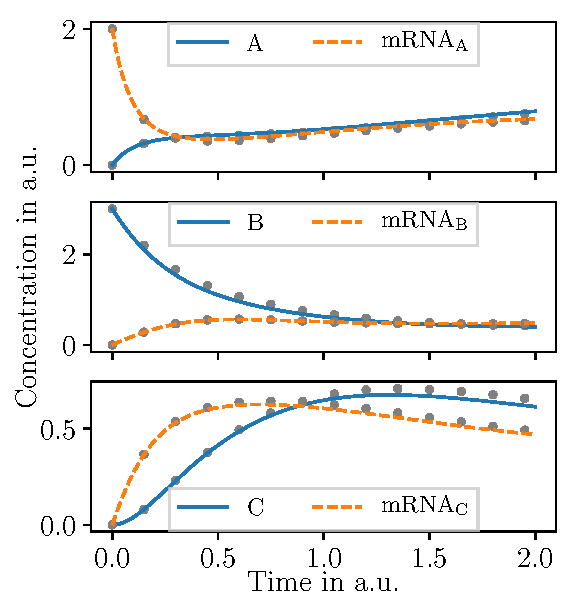
\includegraphics[width=\singlecolumnwidth]{figures_jcp/2.pdf}\caption{\label{fig:case-1-lsq}Concentration time series generated from integrating
the reaction network shown in Fig.~\ref{fig:network}a. The initial
condition prescribes positive concentration values only for $\mathrm{B}$
protein and $\mathrm{mRNA}_{\mathrm{A}}$ species (Tab.~\ref{tab:Initial-conditions}a).
This initial condition is used in the subsequent sections for further
analysis. Gray dots depict concentration time series yielded from
the LSQ rates estimated in Sec~\ref{sec:case-1}.}
\end{figure}

%\ifthisispreprint
% ignore
%\else
%\onecolumngrid
%\fi

\begin{figure*}
\centering 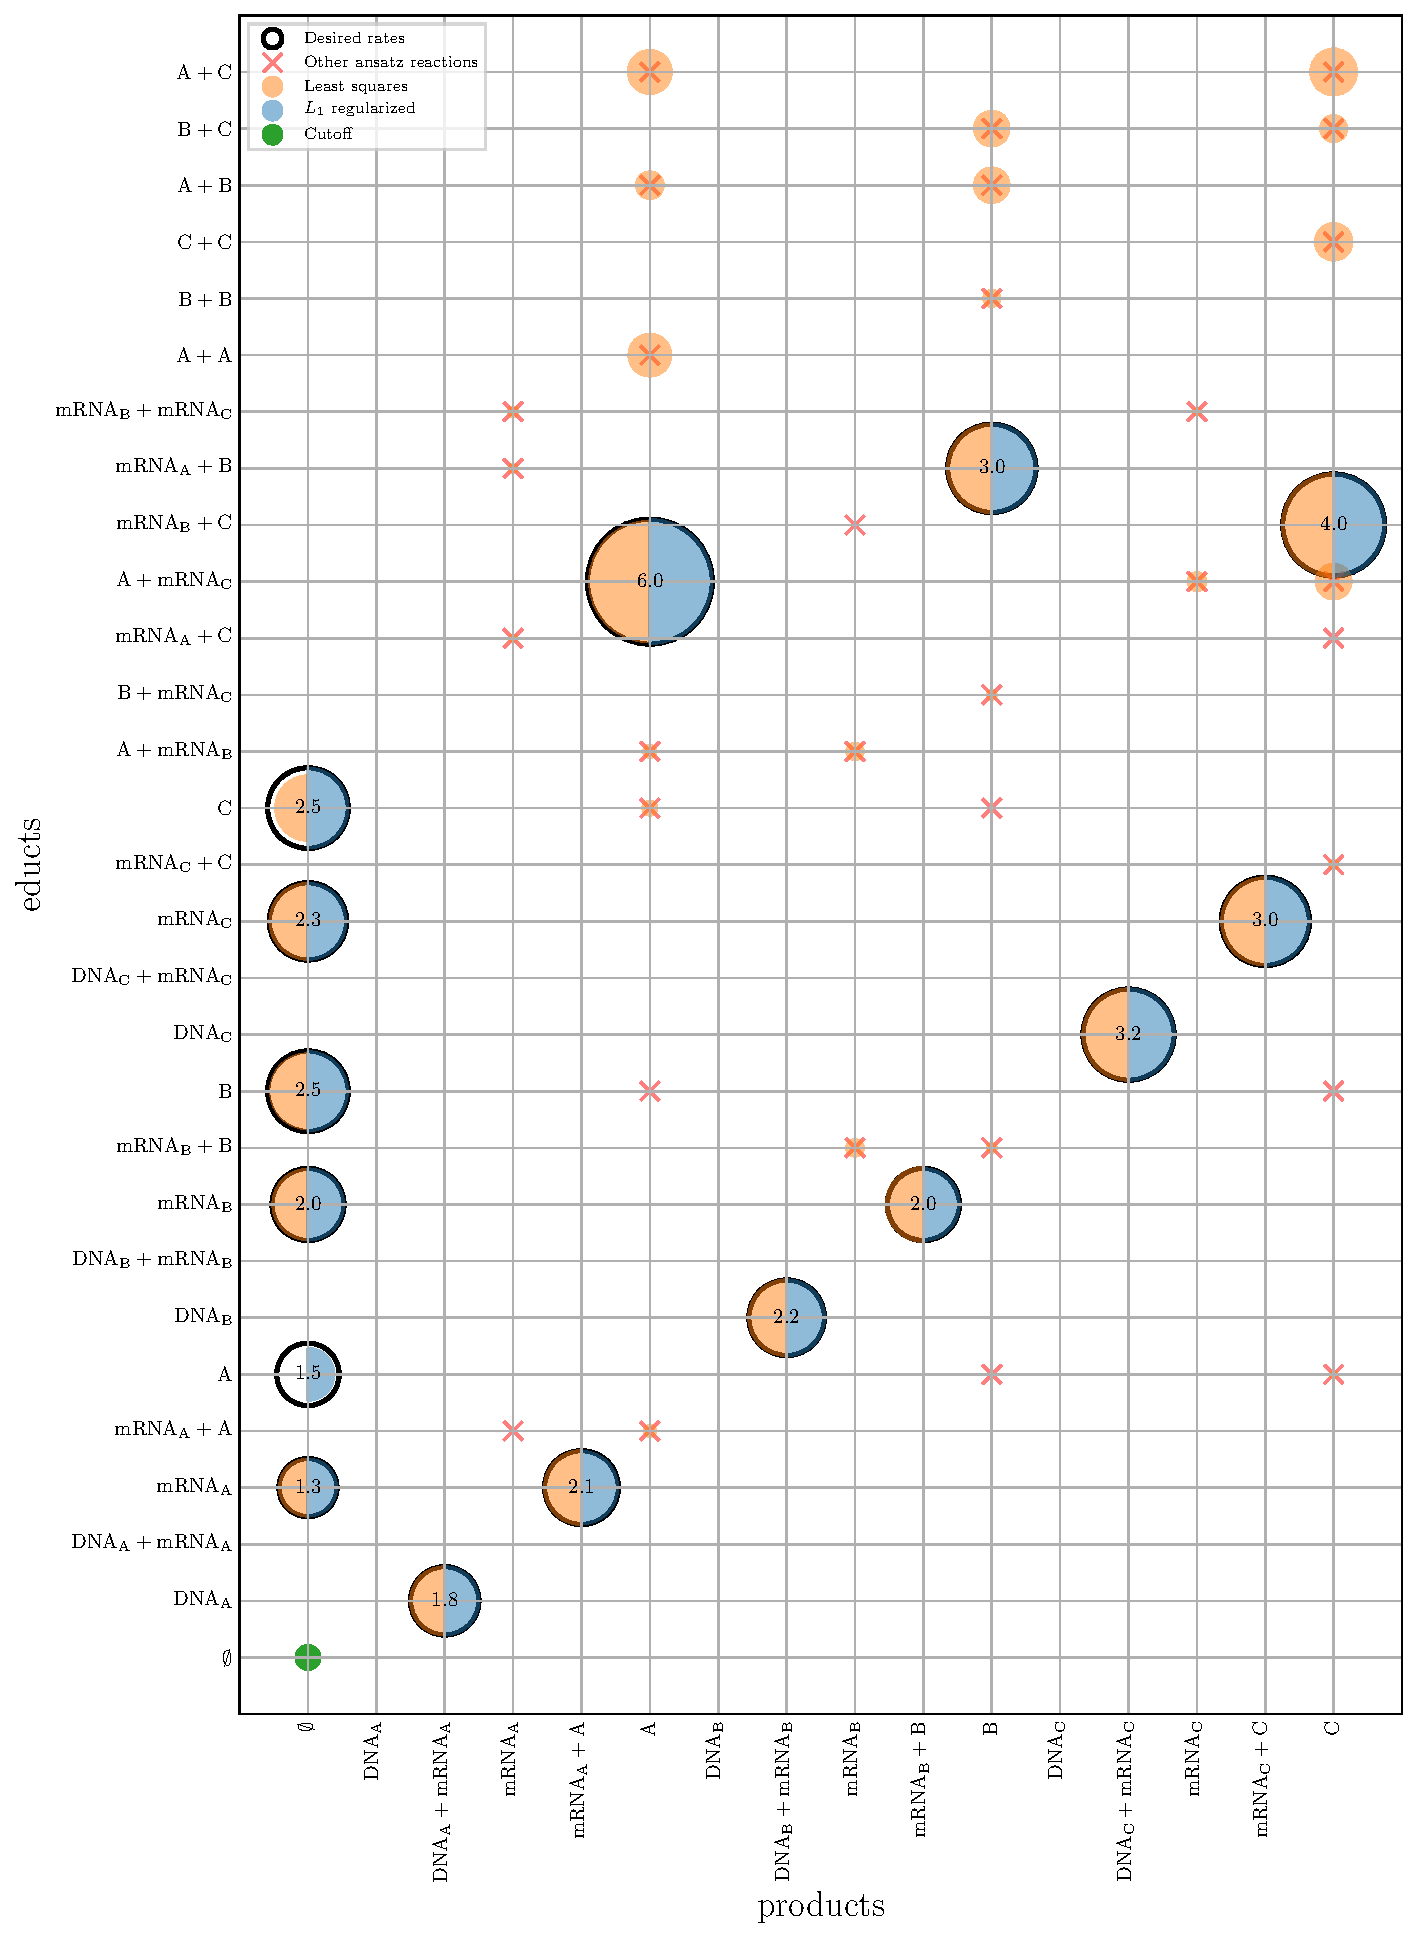
\includegraphics[width=0.82\doublecolumnwidth]{figures_jcp/3.pdf}
\caption{\label{fig:case-1-sparsity-pattern}Estimated reaction rates in the
system described in Sec.~\ref{sec:case-1}. The y and x axes contain
reaction educts and products, respectively. A circle at position $(i,j)$
represents a reaction $i\rightharpoonup j$ whose rate has a linear
relation with the area of the circle. The black outlines denote the
reactions with which the system was generated and contain the respective
rate value. Red crosses denote reactions that were used as additional
ansatz reactions. Blue circles are estimated by LSQ and orange circles
depict rates which were obtained by solving the minimization problem
(\ref{method:minimizationproblem}). The latter rates are subject
to a cutoff $\kappa=0.22$ corresponding to the green circle's area
under which a sparse solution with the correct processes can be recovered.
If a certain rate was estimated in both cases, two wedges instead
of one circle are displayed.}
\end{figure*}
%\ifthisispreprint
% ignore
%\else
%\twocolumngrid
%\fi

Next, we sought sparse solutions by using $\alpha>0$ and additionally
eliminating reactions with rate constants smaller than a cutoff value
$\kappa$. For a suitable choice of hyperparameters $\alpha\approx1.91\cdot10^{-7}$,
$\lambda=1$, and $\kappa=0.22$, a sparse solution is obtained that
finds the correct reaction scheme and also recovers the decay reaction
(Fig.~\ref{fig:case-1-sparsity-pattern}).

The value of the cutoff $\kappa$ was determined by comparing the magnitude
of estimated rates and finding a gap, see Fig.~\ref{fig:reaction-rates-sorted}.
The hyperparameter pair $(\alpha,\lambda)$ was obtained by a grid
search and evaluating the difference $\|\hat{\Xi}_{\alpha,\lambda}-\Xi\|_{1}$,
where $\hat{\Xi}_{\alpha,\lambda}$ is the estimated model under a
particular hyperparameter choice and $\Xi$ is the ground truth. If
the ground truth is unknown, a hyperparameter pair can be estimated
by utilizing cross-validation as in the following sections.


\subsection{Learning the reaction network from data with stochastic noise\label{sec:case-2} }

In contrast to Sec.~\ref{sec:case-1}, we now employ data that includes
measurement noise. Such noise can originate from uncertainties in
the experimental setup or from shot noise in single- or few-molecule
measurements. In gene regulatory networks such noise is commonly observed
when only few copy numbers of $\mathrm{mRNA}$ are present~\cite{Golding2005,Berg1978,Elowitz2002}.
In order to simulate noise from few copies of molecules, the system
of Sec.~\ref{sec:results} with initial conditions as given in Tab.~\ref{tab:Initial-conditions}a
is integrated using the Gillespie stochastic simulation algorithm
(SSA)~\cite{gillespie1976general,gillespie1977exact}. In the limit
of many particles and realizations, the Gillespie SSA converges to
the integrated reaction-rate equations subject to the law of mass
action. As our model is based on exactly these dynamics, the initial
condition's concentrations are interpreted in terms of hundreds of
particles. Each realization is then transformed back to a time series
of concentrations. We define the noise level as the mean-squared deviation
of the concentration time series from the integrated reaction-rate
equations. Data with different noise levels are prepared by averaging
multiple realizations of the time series obtained by the Gillespie
SSA.

It can be observed that decreasing levels of noise lead to fewer spurious
reactions when applying reactive SINDy (\ref{method:minimizationproblem}),
see Fig.~\ref{fig:case2-convergence}a. Also the estimation error
$\|\xi-\hat{\xi}\|_{1}$ with respect to the ground truth $\xi$ decreases
with decreasing levels of noise (Fig.~\ref{fig:case2-convergence}b).
In both cases, the regularized method with a suitable hyperparameter
pair $(\alpha,\lambda)$ performs better than LSQ.

\begin{figure}
\centering 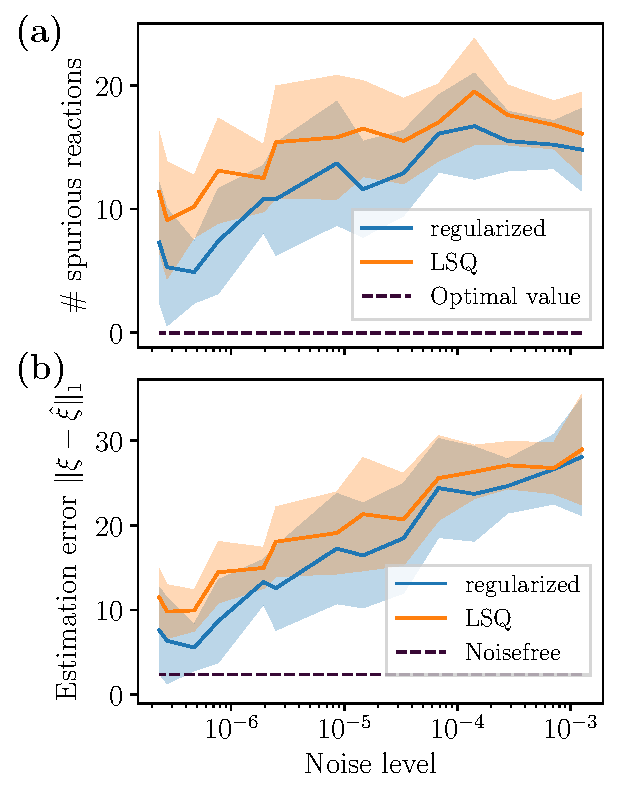
\includegraphics[width=\singlecolumnwidth]{figures_jcp/4.pdf}
\caption{\label{fig:case2-convergence}Convergence of the estimation error
when estimating the system described in Sec.~\ref{sec:case-1} with
varying levels of noise by application of reactive SINDy (\ref{method:minimizationproblem})
with and without regularization in blue and orange, respectively.
The procedure was independently repeated $10$ times with different
realizations giving rise to the mean and standard deviation depicted
by solid lines and shaded areas, respectively. \textbf{(a)}: The number
of detected spurious reactions up to the cutoff value introduced in
Sec.~\ref{sec:case-1} over different levels of noise. \textbf{(b)}:
The estimation error given by the mean absolute error between the
generating reaction rates $\xi$ and the estimated reaction rates
$\hat{\xi}$ over different levels of noise.}
\end{figure}
The hyperparameters $(\alpha,\lambda)$ are obtained by shuffling
the data and performing a $10$-fold cross validation. 

\subsection{Learning the reaction network from multiple initial conditions\label{sec:case-3}}

Preparing the experiment that generates the data in different initial
conditions can help identifying the true reaction mechanisms as a
more diverse dataset makes it easier to confirm or exclude the participation
of specific reactions. This section extends the analysis of Sec.~\ref{sec:case-2}
to two initial conditions, where the first initial condition is identical
to the one used previously and the second initial condition is given
in Tab.~\ref{tab:Initial-conditions}b. 

The corresponding time series are depicted in Fig.~\ref{fig:case3-convergence}a.
The gray graph corresponds to a sample trajectory generated by the
Gillespie SSA. For both initial conditions the same time step of $\tau=3\cdot10^{-3}$
has been applied, amounting to $2\cdot667=1334$ frames. Once the
data matrices 
\[
\mathbf{X}_{1}=\begin{pmatrix}\boldsymbol{x}_{1}(t_{1}) & \cdots & \boldsymbol{x}_{1}(t_{667})\end{pmatrix},\;\mathbf{X}_{2}=\begin{pmatrix}\boldsymbol{x}_{2}(t_{1}) & \cdots & \boldsymbol{x}_{2}(t_{667})\end{pmatrix}
\]
 and the corresponding derivatives $\dot{\mathbf{X}}_{1}$, $\dot{\mathbf{X}}_{2}$
have been obtained, the frames are concatenated so that 
\[
\mathbf{X}=\begin{pmatrix}\boldsymbol{x}_{1}(t_{1}) & \cdots & \boldsymbol{x}_{1}(t_{667}) & \boldsymbol{x}_{2}(t_{1}) & \cdots & \boldsymbol{x}_{2}(t_{667})\end{pmatrix},
\]
analogously for $\dot{\mathbf{X}}$.

Similarly to Sec.~\ref{sec:case-2}, decreasing levels of noise lead
to fewer spurious reactions (Fig.~\ref{fig:case3-convergence}b)
and a smaller $L_{1}$ distance to the ground truth (Fig.~\ref{fig:case3-convergence}c).
Again applying the optimization problem with a suitable set of parameters
$(\alpha,\lambda,\kappa)$ performs better than LSQ. Compared to the
previous section the convergence is better due to twice as much available
data. At noise levels of smaller than roughly $10^{-6}$ the model
can reliably be recovered when using the regularized method.

\begin{figure}
\centering 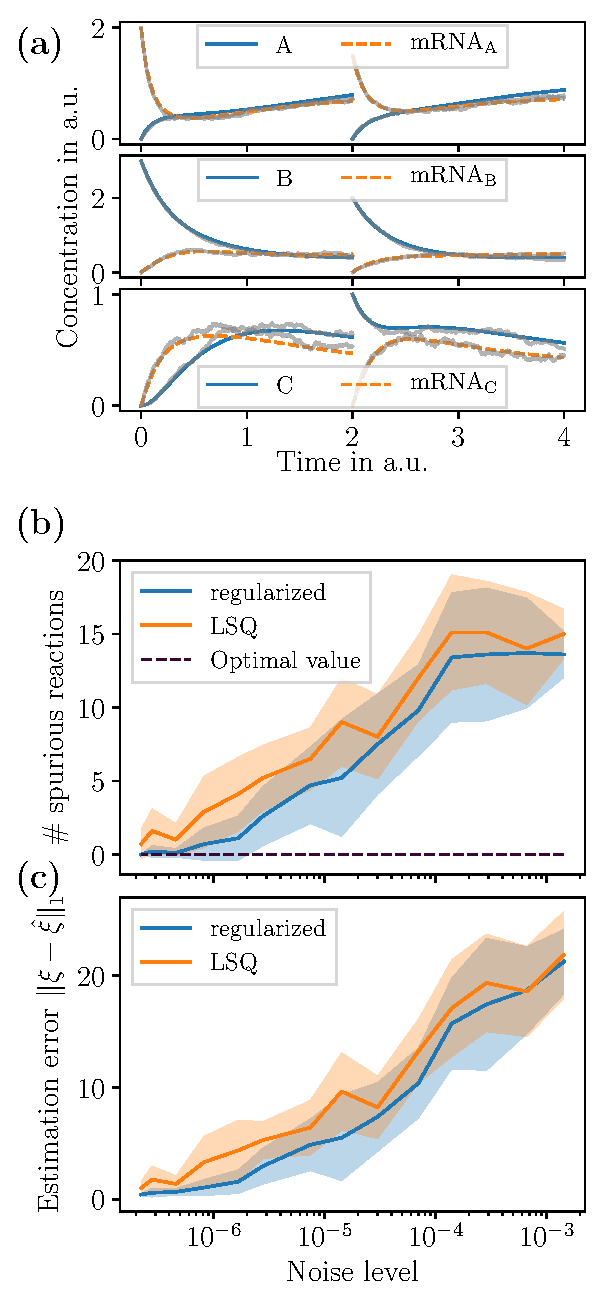
\includegraphics[width=\singlecolumnwidth]{figures_jcp/5.pdf}
\caption{\label{fig:case3-convergence}Convergence of estimation error of reaction
schemes from noisy gene-regulation data starting from two different
initial conditions under decreasing levels of noise. The minimization
problem (\ref{method:minimizationproblem}) was solved for $\alpha=0$
(LSQ) and with regularization. This was repeated $10$ times on different
sets of observation data generated by Gillespie SSA, giving rise to
mean and standard deviation (solid lines and shaded areas, respectively).
\textbf{(a)}: Concentration time series corresponding to the initial
conditions, generated by integrating the reaction-rate equations.
The first initial condition is identical to the one used in Sec.~\ref{sec:case-1}
and Sec.~\ref{sec:case-2}. The second initial condition (Tab.~\ref{tab:Initial-conditions}b)
prescribes positive initial concentrations for $\mathrm{mRNA}_{\mathrm{A}}$,
$\mathrm{B}$, and $\mathrm{C}$ species. The gray graphs are sample
realizations of integration using the Gillespie SSA. \textbf{(b)},\textbf{(c)}:
Analogously to Fig.~\ref{fig:case2-convergence} with the difference
that 20-fold cross validation was used for hyperparameter estimation.}
\end{figure}
The hyperparameters $(\alpha,\lambda)$ are obtained by shuffling
the data and performing a $20$-fold cross validation.

\subsection{Application to MAPK cascade\label{sec:mapk}}
The reactive SINDy method is applied to the mitogen activated protein 
kinases (MAPK) pathway~\cite{Xing1996} which is an important regulatory mechanism of 
biological cells to respond to stimuli and is involved in proliferation, differentiation, 
inflammation, and apoptosis~\cite{Zhang2002mapk}. 
Single-cell MAPK kinetics can be observed experimentally~\cite{Ryu2018integrated}.
Mathematically MAPK kinetics are often modelled using reaction 
rate equations~\cite{Kolch2005kinases,Orton2005computational} which 
enables analysis using reactive SINDy.

Generally a MAPK pathway consists of multiple stages of kinases that 
are either inactive or active, denoted by ``*''. Their activation occurs 
due to phosphorylation catalyzed by the upstream kinase of the previous 
stage, dephosphorylation is catalyzed by phosphatases. When the kinase is 
active it can activate other downstream kinases of the next stage. 
The initial activation is often due to an external stimulus. 
The response of the whole cascade is the amount of activated substrate 
after the final stage, typically measured as a function of the initial stimulus.

Here we model the MAPK pathway with three stages of kinases $\mathrm{MAPK}$, $\mathrm{MAPKK}$, and $\mathrm{MAPKKK}$. The initial stimulus is called $\mathrm{S}$ and the final substrate to be activated is a transcription factor $\mathrm{TF}$. The ground truth reaction network consists of activation/phosphorylation reactions
\begin{align*}
\mathrm{S}        + \mathrm{MAPKKK}  & \rightharpoonup \mathrm{S      } + \mathrm{MAPKKK*} \\
\mathrm{MAPKKK*}  + \mathrm{MAPKK }  & \rightharpoonup \mathrm{MAPKKK*} + \mathrm{MAPKK* } \\
\mathrm{MAPKK*}   + \mathrm{MAPK  }  & \rightharpoonup \mathrm{MAPKK* } + \mathrm{MAPK*  } \\
\mathrm{MAPK*}    + \mathrm{TF    }  & \rightharpoonup \mathrm{MAPK*  } + \mathrm{TF*    } \\
\end{align*}
and deactivation/dephosphorylation reactions
\begin{align*}
\mathrm{MAPKKK*}                     & \rightharpoonup \mathrm{MAPKKK }  \\
\mathrm{MAPKK*}                      & \rightharpoonup \mathrm{MAPKK  }  \\
\mathrm{MAPK*}                       & \rightharpoonup \mathrm{MAPK   }  \\
\mathrm{TF*}                         & \rightharpoonup \mathrm{TF     }.
\end{align*}
For simplicity we assume phosphatase to be abundant such that deactivations 
effectively become first order reactions.
The external stimulus $\mathrm{S}$ is not consumed such that time integration of these 
reactions yields a steady state in which the response, i.e. the concentration $[\mathrm{TF*}]$ 
can be measured as a function of the stimulus concentration $[\mathrm{S}]$.
Using the rate constants given in Tab.~\ref{tab:reaction-library-mapk} we obtain the 
response curve given in Fig.~\ref{fig:mapk}a. 

We generate concentration time series data of the MAPK reactions above at 
three different initial conditions, each differing in the amount of stimulus $[\mathrm{S}]$.
They are marked in Fig.~\ref{fig:mapk}a by vertical dashed lines.
These time series are concatenated to yield a dataset of 300 frames in total.
We use the library $\Theta$ of candidate reactions Tab.~\ref{tab:reaction-library-mapk}.
To determine the hyperparameter $\alpha=6.6\times 10^{-9}$ we shuffle the data and perform
15-fold cross validation. We obtain the estimated 
rate constants by solving the minimization problem (\ref{method:minimizationproblem}) 
with $\lambda=1$. The results are given in Fig.~\ref{fig:mapk}b.
Least-squares estimation detects 5 of the 8 reaction processes that belong to the 
ground truth model. However it also detects 12 other reaction 
processes ($\theta_{18}$ - $\theta_{29}$) which are not in the ground truth.
Reactive SINDy estimation detects all reactions of the ground truth, 
two processes ($\theta_{4}$ and $\theta_{8}$) show deviations in 
rate constants. Generally reactive SINDy yields a sparse model which allows further
simplification of the reaction network by dropping out reaction processes that lie 
beneath a certain cutoff. In this case for example a cutoff of $0.25$ would directly recover
the ground truth reaction network.
Quantitatively, one may consider the $L_1$ norm of the relative distance 
of estimated rate constants $\hat{\xi}_r$ to the non-zero rate 
constants of the ground truth $\xi_r$
\begin{equation*}
\sum_{r=1}^{8} \left|(\hat{\xi}_{r} - \xi_r)/\xi_r\right|
\end{equation*}
which yields $167\%$ error for least-squares and $21\%$ error for reactive SINDy.

\begin{figure}
    \centering
    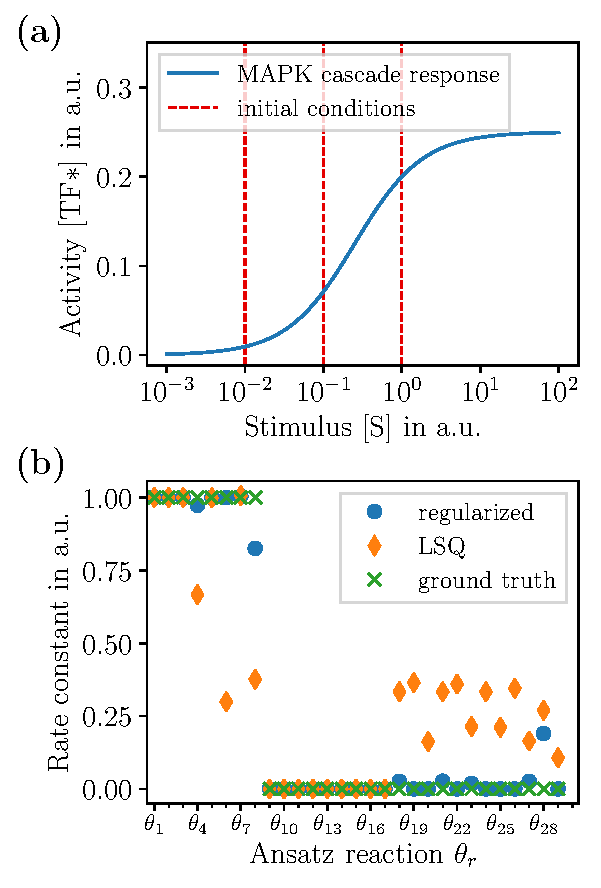
\includegraphics[width=\singlecolumnwidth]{figures_jcp/6.pdf}
    \caption{\label{fig:mapk}Application of reactive SINDy to the MAPK pathway system. \textbf{(a)}~The response curve of the MAPK cascade as a function of external stimulus given as a constant concentration $[\mathrm{S}]$. The activity is the steady state concentration of activated transcription factors $[\mathrm{TF*}]$. Dashed lines show the values of $[\mathrm{S}]$ at which concentration time series data was generated. \textbf{(b)}~Estimated rate coefficients of candidate reactions (see Tab.~\ref{tab:reaction-library-mapk}) after application of reactive SINDy (regularized) to the time series data. Least-squares estimation (LSQ) and the ground truth model for comparison.}
\end{figure}

\subsection{Application to Lotka-Volterra system\label{sec:lv}}
As biological pathways often exhibit oscillatory behavior~\cite{Iqbal2008tnf} which can stem 
from positive or negative feedback loops~\cite{Shin2009positive} we apply reactive SINDy to
an idealized oscillatory system, namely the Lotka-Volterra system. 
The predator-prey dynamics of two species $\mathrm{A}$ (prey) and $\mathrm{B}$ 
(predator) is defined by the reactions
\begin{align*}
\mathrm{A}              & \rightharpoonup \mathrm{A} + \mathrm{A} &  & \text{(prey growth)},\\
\mathrm{A} + \mathrm{B} & \rightharpoonup \mathrm{B} + \mathrm{B} &  & \text{(predator eats prey)},\\
\mathrm{B}              & \rightharpoonup \emptyset &  & \text{(predator decay)},\\
\mathrm{A} + \mathrm{A} & \rightharpoonup \emptyset &  & \text{(prey friction)},\\
\mathrm{B} + \mathrm{B} & \rightharpoonup \emptyset &  & \text{(predator friction)}.
\end{align*}
From this model we generate concentration time series data with $200$ frames 
which is displayed in Fig.~\ref{fig:lv}a. We construct the library $\Theta$ 
of candidate reactions given in Tab.~\ref{tab:reaction-library-lv}. 
We determine the hyperparameter $\alpha=2.7\times10^{-7}$ by shuffling 
the data and performing 5-fold cross validation. We obtain the estimated 
rate constants by solving the minimization problem (\ref{method:minimizationproblem}) 
with $\lambda=1$. The results are given in Fig.~\ref{fig:lv}b.
Least-squares estimation detects all reactions of the ground truth model but also
two false processes ($\theta_{6}$ and $\theta_{7}$) with a higher rate than
the two first true processes ($\theta_{1}$ and $\theta_{2}$). Reactive SINDy detects
the true reaction network with minor deviations in rate constants. As in 
Sec.~\ref{sec:mapk} we consider the $L_1$ norm of the relative distance to the ground truth
for non-zero rate constants
\begin{equation*}
\sum_{r=1}^{5} \left|(\hat{\xi}_{r} - \xi_r)/\xi_r\right|
\end{equation*}
which yields $75\%$ error for least-squares and $7\%$ error for reactive SINDy.

\begin{figure}
    \centering
    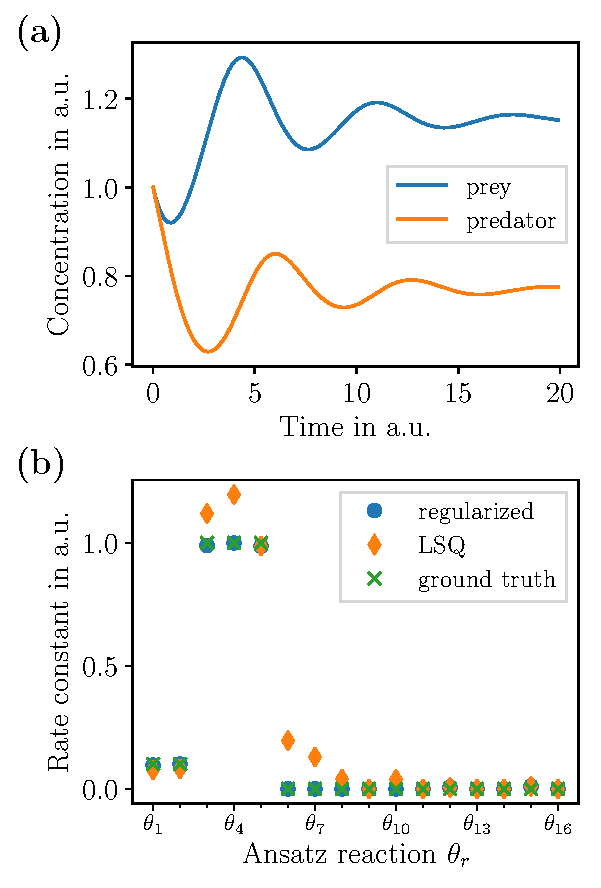
\includegraphics[width=\singlecolumnwidth]{figures_jcp/7.pdf}
    \caption{\label{fig:lv}Application of reactive SINDy to the Lotka-Volterra system with social friction. \textbf{(a)}~Concentration data as a function of time for predator and prey species. \textbf{(b)}~Estimated rate coefficients of candidate reactions (see Tab.~\ref{tab:reaction-library-lv}) after application of reactive SINDy (regularized) to the time series data. Least-squares estimation (LSQ) estimation and the ground truth model for comparison.}
\end{figure}

\section{Conclusion}

In this work we have extended the SINDy method to reactive SINDy,
not only parsimoniously detecting potentially nonlinear terms in a
dynamical system from noisy data, but also yielding, in this case,
a sparse set of rates with respect to generating reactions (\ref{method:the-reactions}).
Mathematically this has been achieved by permitting vector-valued
basis functions and obtaining a tensor linear regression problem.
We have applied this method on data generated from a gene regulation
network, a MAPK pathway, and a Lotka-Volterra system and 
could successfully recover the underlying reaction networks.

The studies of Sec.~\ref{sec:case-2} and Sec.~\ref{sec:case-3}
have shown that the applied regularization terms can mitigate noise
up to a certain degree compared to the unregularized method, so that
identification of the reaction network is more robust and closer to
the ground truth.
Potentially, this method could be used to identify reaction networks
from time series measurements even if the initial conditions are not
always exactly identical, as was demonstrated in Sec.~\ref{sec:case-3}.

One apparent limitation is that the method can only be applied if
the data stems from the equilibration phase, as the concentration-based
approach has derivatives equal zero in the equilibrium, which precludes
the reaction dynamics to be recovered. Thus, in the case of oscillatory 
systems the reaction network can be recovered robustly.

In future work, we will consider
the identification of reaction schemes from instantaneous fluctuations
of particle numbers in equilibrium.

\section*{Acknowledgments}

The authors are grateful to the Center for Theoretical Biological
Physics (CTBP, supported by NSF PHY-1427654) at Rice University for
hosting their sabbatical visit, during which part of this work was
performed. 

We gratefully acknowledge funding from Deutsche Forschungsgemeinschaft
(SFB 958 / Project A04, TRR 186 / Project A12, SFB 1114 / Project
C03), Einstein Foundation Berlin (ECMath Project CH17) and European
Research Council (ERC CoG 772230 ``ScaleCell''). We are grateful
for inspiring discussions with Simon Olsson, Mohsen
Sadeghi, Felix Höfling and Christof Schütte.

\section{Appendix\label{sec:appendix}}
\begin{figure}[h!]

\centering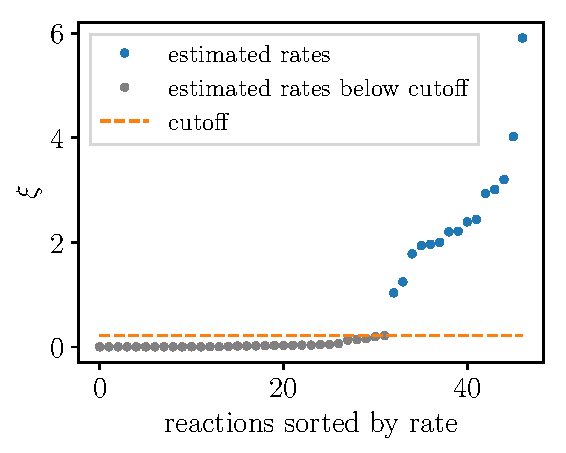
\includegraphics[width=\singlecolumnwidth]{figures_jcp/8.pdf}\caption{\label{fig:reaction-rates-sorted}Reaction rates sorted by their magnitude
to determine the cutoff $\kappa=0.22$ of Sec.~\ref{sec:case-1}.
The rates were estimated using the regularized minimization problem.}

\end{figure}

%\ifthisispreprint
% ignore
%\else
%\onecolumngrid
%\fi

\begin{table*}[h!]
\centering %
%\resizebox{.9\textwidth}{!}{%
\begin{tabular}{rclcc}
\toprule 
\multicolumn{3}{c}{Reaction} & rate  & description \tabularnewline
\midrule 
$\mathrm{DNA}_{\mathrm{A}}$  & $\rightharpoonup$  & $\mathrm{DNA}_{\mathrm{A}}+\mathrm{mRNA}_{\mathrm{A}}$  & $k_{1}=1.8$  & transcription of $\mathrm{mRNA}_{\mathrm{A}}$\tabularnewline
$\mathrm{mRNA}_{\mathrm{A}}$  & $\rightharpoonup$  & $\mathrm{mRNA}_{\mathrm{A}}+\mathrm{A}$  & $k_{2}=2.1$  & translation of $\mathrm{A}$ proteins\tabularnewline
$\mathrm{mRNA}_{\mathrm{A}}$  & $\rightharpoonup$  & $\emptyset$  & $k_{3}=1.3$  & $\mathrm{mRNA}_{\mathrm{A}}$ decay\tabularnewline
$\mathrm{A}$  & $\rightharpoonup$  & $\emptyset$  & $k_{4}=1.5$  & decay of $\mathrm{A}$ proteins\tabularnewline
$\mathrm{DNA}_{\mathrm{B}}$  & $\rightharpoonup$  & $\mathrm{DNA}_{\mathrm{B}}+\mathrm{mRNA}_{\mathrm{B}}$  & $k_{5}=2.2$  & transcription of $\mathrm{mRNA}_{\mathrm{B}}$\tabularnewline
$\mathrm{mRNA}_{\mathrm{B}}$  & $\rightharpoonup$  & $\mathrm{mRNA}_{\mathrm{B}}+\mathrm{B}$  & $k_{6}=2.0$  & translation of $\mathrm{B}$ proteins\tabularnewline
$\mathrm{mRNA}_{\mathrm{B}}$  & $\rightharpoonup$  & $\emptyset$  & $k_{7}=2.0$  & $\mathrm{mRNA}_{\mathrm{B}}$ decay\tabularnewline
$\mathrm{B}$  & $\rightharpoonup$  & $\emptyset$  & $k_{8}=2.5$  & decay of $\mathrm{B}$ proteins\tabularnewline
$\mathrm{DNA}_{\mathrm{C}}$  & $\rightharpoonup$  & $\mathrm{DNA}_{\mathrm{C}}+\mathrm{mRNA}_{\mathrm{C}}$  & $k_{9}=3.2$  & transcription of $\mathrm{mRNA}_{\mathrm{C}}$\tabularnewline
$\mathrm{mRNA}_{\mathrm{C}}$  & $\rightharpoonup$  & $\mathrm{mRNA}_{\mathrm{C}}+\mathrm{C}$  & $k_{10}=3.0$  & translation of $\mathrm{C}$ proteins\tabularnewline
$\mathrm{mRNA}_{\mathrm{C}}$  & $\rightharpoonup$  & $\emptyset$  & $k_{11}=2.3$  & $\mathrm{mRNA}_{\mathrm{C}}$ decay\tabularnewline
$\mathrm{C}$  & $\rightharpoonup$  & $\emptyset$  & $k_{12}=2.5$  & decay of $\mathrm{C}$ proteins\tabularnewline
$\mathrm{mRNA}_{\mathrm{A}}+\mathrm{A}$  & $\rightharpoonup$  & $\mathrm{A}$  & $k_{13}=0$  & self regulation of $\mathrm{A}$ proteins\tabularnewline
$\mathrm{mRNA}_{\mathrm{B}}+\mathrm{B}$  & $\rightharpoonup$  & $\mathrm{B}$  & $k_{14}=0$  & self regulation of $\mathrm{B}$ proteins\tabularnewline
$\mathrm{mRNA}_{\mathrm{C}}+\mathrm{C}$  & $\rightharpoonup$  & $\mathrm{C}$  & $k_{15}=0$  & self regulation of $\mathrm{C}$ proteins\tabularnewline
$\mathrm{mRNA}_{\mathrm{B}}+\mathrm{A}$  & $\rightharpoonup$  & $\mathrm{A}$  & $k_{16}=0$  & regulation of $\mathrm{mRNA}_{\mathrm{B}}$\tabularnewline
$\mathrm{mRNA}_{\mathrm{C}}+\mathrm{B}$  & $\rightharpoonup$  & $\mathrm{B}$  & $k_{17}=0$  & regulation of $\mathrm{mRNA}_{\mathrm{C}}$\tabularnewline
$\mathrm{mRNA}_{\mathrm{A}}+\mathrm{C}$  & $\rightharpoonup$  & $\mathrm{C}$  & $k_{18}=0$  & regulation of $\mathrm{mRNA}_{\mathrm{A}}$\tabularnewline
$\mathrm{mRNA}_{\mathrm{C}}+\mathrm{A}$  & $\rightharpoonup$  & $\mathrm{A}$  & $k_{16}=6.0$  & regulation of $\mathrm{mRNA}_{\mathrm{C}}$\tabularnewline
$\mathrm{mRNA}_{\mathrm{B}}+\mathrm{C}$  & $\rightharpoonup$  & $\mathrm{C}$  & $k_{17}=4.0$  & regulation of $\mathrm{mRNA}_{\mathrm{B}}$\tabularnewline
$\mathrm{mRNA}_{\mathrm{A}}+\mathrm{B}$  & $\rightharpoonup$  & $\mathrm{B}$  & $k_{18}=3.0$  & regulation of $\mathrm{mRNA}_{\mathrm{A}}$\tabularnewline
$\mathrm{mRNA}_{\mathrm{A}}+\mathrm{A}$  & $\rightharpoonup$  & $\mathrm{mRNA}_{\mathrm{A}}$  & $k_{19}=0$  & artificial fusion\tabularnewline
$\mathrm{mRNA}_{\mathrm{B}}+\mathrm{B}$  & $\rightharpoonup$  & $\mathrm{mRNA}_{\mathrm{B}}$  & $k_{20}=0$  & artificial fusion\tabularnewline
$\mathrm{mRNA}_{\mathrm{A}}+\mathrm{B}$  & $\rightharpoonup$  & $\mathrm{mRNA}_{\mathrm{A}}$  & $k_{21}=0$  & artificial fusion\tabularnewline
$\mathrm{mRNA}_{\mathrm{B}}+\mathrm{C}$  & $\rightharpoonup$  & $\mathrm{mRNA}_{\mathrm{B}}$  & $k_{22}=0$  & artificial fusion\tabularnewline
$\mathrm{mRNA}_{\mathrm{C}}+\mathrm{A}$  & $\rightharpoonup$  & $\mathrm{mRNA}_{\mathrm{C}}$  & $k_{23}=0$  & artificial fusion\tabularnewline
$\mathrm{mRNA}_{\mathrm{A}}+\mathrm{C}$  & $\rightharpoonup$  & $\mathrm{mRNA}_{\mathrm{A}}$  & $k_{24}=0$  & artificial fusion\tabularnewline
$\mathrm{mRNA}_{\mathrm{B}}+\mathrm{A}$  & $\rightharpoonup$  & $\mathrm{mRNA}_{\mathrm{B}}$  & $k_{25}=0$  & artificial fusion\tabularnewline
$\mathrm{A}+\mathrm{A}$  & $\rightharpoonup$  & $\mathrm{A}$  & $k_{26}=0$  & $\mathrm{A}$ regulates $\mathrm{A}$\tabularnewline
$\mathrm{B}+\mathrm{B}$  & $\rightharpoonup$  & $\mathrm{B}$  & $k_{27}=0$  & $\mathrm{B}$ regulates $\mathrm{B}$\tabularnewline
$\mathrm{C}+\mathrm{C}$  & $\rightharpoonup$  & $\mathrm{C}$  & $k_{28}=0$  & $\mathrm{C}$ regulates $\mathrm{C}$\tabularnewline
$\mathrm{B}+\mathrm{A}$  & $\rightharpoonup$  & $\mathrm{A}$  & $k_{29}=0$  & artificial fusion\tabularnewline
$\mathrm{C}+\mathrm{B}$  & $\rightharpoonup$  & $\mathrm{B}$  & $k_{30}=0$  & artificial fusion\tabularnewline
$\mathrm{A}+\mathrm{C}$  & $\rightharpoonup$  & $\mathrm{C}$  & $k_{31}=0$  & artificial fusion\tabularnewline
$\mathrm{C}+\mathrm{A}$  & $\rightharpoonup$  & $\mathrm{A}$  & $k_{32}=0$  & artificial fusion\tabularnewline
$\mathrm{B}+\mathrm{C}$  & $\rightharpoonup$  & $\mathrm{C}$  & $k_{33}=0$  & artificial fusion\tabularnewline
$\mathrm{A}+\mathrm{B}$  & $\rightharpoonup$  & $\mathrm{B}$  & $k_{34}=0$  & artificial fusion\tabularnewline
$\mathrm{A}$  & $\rightharpoonup$  & $\mathrm{B}$  & $k_{35}=0$  & artificial conversion\tabularnewline
$\mathrm{B}$  & $\rightharpoonup$  & $\mathrm{C}$  & $k_{36}=0$  & artificial conversion\tabularnewline
$\mathrm{C}$  & $\rightharpoonup$  & $\mathrm{A}$  & $k_{37}=0$  & artificial conversion\tabularnewline
$\mathrm{A}$  & $\rightharpoonup$  & $\mathrm{C}$  & $k_{38}=0$  & artificial conversion\tabularnewline
$\mathrm{C}$  & $\rightharpoonup$  & $\mathrm{B}$  & $k_{39}=0$  & artificial conversion\tabularnewline
$\mathrm{B}$  & $\rightharpoonup$  & $\mathrm{A}$  & $k_{40}=0$  & artificial conversion\tabularnewline
$\mathrm{mRNA}_{\mathrm{B}}+\mathrm{mRNA}_{\mathrm{C}}$  & $\rightharpoonup$  & $\mathrm{mRNA}_{\mathrm{A}}$  & $k_{41}=0$  & artificial fusion\tabularnewline
$\mathrm{mRNA}_{\mathrm{C}}+\mathrm{mRNA}_{\mathrm{B}}$  & $\rightharpoonup$  & $\mathrm{mRNA}_{\mathrm{C}}$  & $k_{42}=0$  & artificial fusion\tabularnewline
$\mathrm{mRNA}_{\mathrm{C}}+\mathrm{A}$  & $\rightharpoonup$  & $\mathrm{C}$  & $k_{43}=0$  & artificial fusion\tabularnewline
\bottomrule
\end{tabular}\caption{\label{tab:reaction-library}Full set of ansatz reactions $\Theta$ used in Sec.~\ref{sec:results} for the gene-regulatory network. The given rate constants define the ground truth reaction model.}
\end{table*}

\begin{table*}[h!]
    \centering %
    %\resizebox{.9\textwidth}{!}{%
    \begin{tabular}{rclcc}
        \toprule 
        \multicolumn{3}{c}{Reaction} & rate & description \tabularnewline
        \midrule 
        $\mathrm{S}        + \mathrm{MAPKKK}$  & $\rightharpoonup$  &  $\mathrm{S      } + \mathrm{MAPKKK*}$ & $k_{1} =1$ & external stimulus activates MAPKKK\tabularnewline
        $\mathrm{MAPKKK*}    \mathrm{      }$  & $\rightharpoonup$  &  $\mathrm{MAPKKK }                   $ & $k_{2} =1$ & dephosphorylation\tabularnewline
        $\mathrm{MAPKKK*}  + \mathrm{MAPKK }$  & $\rightharpoonup$  &  $\mathrm{MAPKKK*} + \mathrm{MAPKK* }$ & $k_{3} =1$ & phosphorylation of MAPKK\tabularnewline
        $\mathrm{MAPKK*}     \mathrm{      }$  & $\rightharpoonup$  &  $\mathrm{MAPKK  }                   $ & $k_{4} =1$ & dephosphorylation\tabularnewline
        $\mathrm{MAPKK*}   + \mathrm{MAPK  }$  & $\rightharpoonup$  &  $\mathrm{MAPKK* } + \mathrm{MAPK*  }$ & $k_{5} =1$ & phosphorylation of MAPK\tabularnewline
        $\mathrm{MAPK*}      \mathrm{      }$  & $\rightharpoonup$  &  $\mathrm{MAPK   }                   $ & $k_{6} =1$ & dephosphorylation\tabularnewline
        $\mathrm{MAPK*}    + \mathrm{TF    }$  & $\rightharpoonup$  &  $\mathrm{MAPK*  } + \mathrm{TF*    }$ & $k_{7} =1$ & phosphorylation of transcription factor\tabularnewline
        $\mathrm{TF*}        \mathrm{      }$  & $\rightharpoonup$  &  $\mathrm{TF     }                   $ & $k_{8} =1$ & dephosphorylation\tabularnewline
        $\mathrm{MAPKKK}   + \mathrm{MAPKK }$  & $\rightharpoonup$  &  $\mathrm{MAPKKK } + \mathrm{MAPKK* }$ & $k_{9} =0$ & artificial reaction\tabularnewline
        $\mathrm{MAPKKK}   + \mathrm{MAPK  }$  & $\rightharpoonup$  &  $\mathrm{MAPK*  }                   $ & $k_{10}=0$ & artificial reaction\tabularnewline
        $\mathrm{MAPKKK}   + \mathrm{TF    }$  & $\rightharpoonup$  &  $\mathrm{MAPKKK } + \mathrm{TF*    }$ & $k_{11}=0$ & artificial reaction\tabularnewline
        $\mathrm{MAPKKK*}  + \mathrm{MAPK  }$  & $\rightharpoonup$  &  $\mathrm{MAPKKK*} + \mathrm{MAPK*  }$ & $k_{12}=0$ & artificial reaction\tabularnewline
        $\mathrm{MAPKKK*}  + \mathrm{TF    }$  & $\rightharpoonup$  &  $\mathrm{MAPKKK*} + \mathrm{TF*    }$ & $k_{13}=0$ & artificial reaction\tabularnewline
        $\mathrm{MAPKK}    + \mathrm{TF    }$  & $\rightharpoonup$  &  $\mathrm{MAPKK  } + \mathrm{TF*    }$ & $k_{14}=0$ & artificial reaction\tabularnewline
        $\mathrm{MAPKK*}   + \mathrm{TF    }$  & $\rightharpoonup$  &  $\mathrm{MAPKK* } + \mathrm{TF*    }$ & $k_{15}=0$ & artificial reaction\tabularnewline
        $\mathrm{MAPK}     + \mathrm{TF    }$  & $\rightharpoonup$  &  $\mathrm{MAPK   } + \mathrm{TF*    }$ & $k_{16}=0$ & artificial reaction\tabularnewline
        $\mathrm{MAPKK}    + \mathrm{MAPK  }$  & $\rightharpoonup$  &  $\mathrm{MAPKK  } + \mathrm{MAPK*  }$ & $k_{17}=0$ & artificial reaction\tabularnewline
        $\mathrm{MAPKKK}   + \mathrm{MAPKK*}$  & $\rightharpoonup$  &  $\mathrm{MAPKKK } + \mathrm{MAPKK  }$ & $k_{18}=0$ & artificial reaction\tabularnewline
        $\mathrm{MAPKKK}   + \mathrm{MAPK* }$  & $\rightharpoonup$  &  $\mathrm{MAPKKK } + \mathrm{MAPK   }$ & $k_{19}=0$ & artificial reaction\tabularnewline
        $\mathrm{MAPKKK}   + \mathrm{TF*   }$  & $\rightharpoonup$  &  $\mathrm{MAPKKK } + \mathrm{TF     }$ & $k_{20}=0$ & artificial reaction\tabularnewline
        $\mathrm{MAPKKK*}  + \mathrm{MAPKK*}$  & $\rightharpoonup$  &  $\mathrm{MAPKKK*} + \mathrm{MAPKK  }$ & $k_{21}=0$ & artificial reaction\tabularnewline
        $\mathrm{MAPKKK*}  + \mathrm{MAPK* }$  & $\rightharpoonup$  &  $\mathrm{MAPKKK*} + \mathrm{MAPK   }$ & $k_{22}=0$ & artificial reaction\tabularnewline
        $\mathrm{MAPKKK*}  + \mathrm{TF*   }$  & $\rightharpoonup$  &  $\mathrm{MAPKKK*} + \mathrm{TF     }$ & $k_{23}=0$ & artificial reaction\tabularnewline
        $\mathrm{MAPKK}    + \mathrm{MAPK* }$  & $\rightharpoonup$  &  $\mathrm{MAPKK  } + \mathrm{MAPK   }$ & $k_{24}=0$ & artificial reaction\tabularnewline
        $\mathrm{MAPKK}    + \mathrm{TF*   }$  & $\rightharpoonup$  &  $\mathrm{MAPKK  } + \mathrm{TF     }$ & $k_{25}=0$ & artificial reaction\tabularnewline
        $\mathrm{MAPKK*}   + \mathrm{MAPK* }$  & $\rightharpoonup$  &  $\mathrm{MAPKK* } + \mathrm{MAPK   }$ & $k_{26}=0$ & artificial reaction\tabularnewline
        $\mathrm{MAPKK*}   + \mathrm{TF*   }$  & $\rightharpoonup$  &  $\mathrm{MAPKK* } + \mathrm{TF     }$ & $k_{27}=0$ & artificial reaction\tabularnewline
        $\mathrm{MAPK}     + \mathrm{TF*   }$  & $\rightharpoonup$  &  $\mathrm{MAPK   } + \mathrm{TF     }$ & $k_{28}=0$ & artificial reaction\tabularnewline
        $\mathrm{MAPK*}    + \mathrm{TF*   }$  & $\rightharpoonup$  &  $\mathrm{MAPK*  } + \mathrm{TF     }$ & $k_{29}=0$ & artificial reaction\tabularnewline
        \bottomrule
    \end{tabular}\caption{\label{tab:reaction-library-mapk}Full set of ansatz reactions $\Theta$ used in Sec.~\ref{sec:mapk} for the MAPK system. The given rate constants define the ground truth reaction model.}
\end{table*}

\begin{table*}[h!]
    \centering %
    %\resizebox{.9\textwidth}{!}{%
    \begin{tabular}{rclcc}
        \toprule 
        \multicolumn{3}{c}{Reaction} & rate & description \tabularnewline
        \midrule 
        $\mathrm{A} + \mathrm{A}$ & $\rightharpoonup$ & $\emptyset             $  & $k_{1} =0.1$ & social friction of prey\tabularnewline
        $\mathrm{B} + \mathrm{B}$ & $\rightharpoonup$ & $\emptyset             $  & $k_{2} =0.1$ & social friction of predator\tabularnewline
        $\mathrm{A}             $ & $\rightharpoonup$ & $\mathrm{A} + \mathrm{A}$ & $k_{3} =1  $ & prey growth\tabularnewline
        $\mathrm{A} + \mathrm{B}$ & $\rightharpoonup$ & $\mathrm{B} + \mathrm{B}$ & $k_{4} =1  $ & predator eats prey\tabularnewline
        $\mathrm{B}             $ & $\rightharpoonup$ & $\emptyset             $  & $k_{5} =1  $ & predator decays\tabularnewline
        $\mathrm{A} + \mathrm{B}$ & $\rightharpoonup$ & $\mathrm{A} + \mathrm{A}$ & $k_{6} =0  $ & artificial reaction\tabularnewline
        $\mathrm{A}             $ & $\rightharpoonup$ & $\emptyset             $  & $k_{7} =0  $ & artificial reaction\tabularnewline
        $\mathrm{B} + \mathrm{B}$ & $\rightharpoonup$ & $\mathrm{B}             $ & $k_{8} =0  $ & artificial reaction\tabularnewline
        $\mathrm{B}             $ & $\rightharpoonup$ & $\mathrm{B} + \mathrm{B}$ & $k_{9} =0  $ & artificial reaction\tabularnewline
        $\mathrm{A} + \mathrm{A}$ & $\rightharpoonup$ & $\mathrm{A}             $ & $k_{10}=0  $ & artificial reaction\tabularnewline
        $\mathrm{A} + \mathrm{B}$ & $\rightharpoonup$ & $\mathrm{A}             $ & $k_{11}=0  $ & artificial reaction\tabularnewline
        $\mathrm{A} + \mathrm{B}$ & $\rightharpoonup$ & $\mathrm{B}             $ & $k_{12}=0  $ & artificial reaction\tabularnewline
        $\mathrm{A} + \mathrm{A}$ & $\rightharpoonup$ & $\mathrm{B}             $ & $k_{13}=0  $ & artificial reaction\tabularnewline
        $\mathrm{A}             $ & $\rightharpoonup$ & $\mathrm{B}             $ & $k_{14}=0  $ & artificial reaction\tabularnewline
        $\mathrm{B}             $ & $\rightharpoonup$ & $\mathrm{A}             $ & $k_{15}=0  $ & artificial reaction\tabularnewline
        $\mathrm{A}             $ & $\rightharpoonup$ & $\mathrm{B} + \mathrm{B}$ & $k_{16}=0  $ & artificial reaction\tabularnewline
        \bottomrule
    \end{tabular}\caption{\label{tab:reaction-library-lv}Full set of ansatz reactions $\Theta$ used in Sec.~\ref{sec:lv} for the Lotka-Volterra system. The given rate constants define the ground truth reaction model.}
\end{table*}

%\ifthisispreprint
% ignore
%\else
%\twocolumngrid
%\fi

\linespread{1.45}

\clearpage
\newpage{}  \bibliographystyle{abbrv}
\bibliography{bibliography}
\newpage{}

\end{document}
